\chapter{Model symulacyjny}
\label{cha:ch4_model_symulacyjny}

Do zaprojektowania odpowiedniego układu regulacji systemem kulka i belka, a więc dobrania struktury regulatorów, konieczne jest posiadanie modelu tego systemu. Jest to jednak zadanie utrudnione, gdy system jest wybitnie nieliniowy --- a obiekt regulacji taki właśnie jest, gdyż zawiera nieliniowości wynikające z:
\begin{itemize}
    \item przeniesienia napędu poprzez przekładnię korbową,
    \item wynikającej z tego przeniesienia zależności obrotu belki od obrotu silnika,
    \item czy z obecnego w przekładni zastosowanego silnika tarcia suchego.
%    \item dzia.
\end{itemize}

Wobec tego zdecydowano się nie przystępować do opisu matematycznego zachowania się układu w sposób klasyczny, np. poprzez równania Eulera--Lagrange'a czy funkcjonał Hamiltona. Zamiast tego, wykorzystując narzędzia pakietu \textsc{Matlab/Simulink}, zbudowano przestrzenną i fizyczną reprezentację obiektu regulacji, która następnie została wykorzystana do linearyzacji i dobrania regulatorów (rozdział \ref{cha:ch6_model_liniowy}).

\section{Wykorzystanie przybornika \textsc{Simscape Multibody}}
\label{sec:ch4_simmechanics}

\textsc{Simscape Multibody}, znany również jako \textsc{SimMechanics}, pozwala na modelowanie fizycznych układów (ciał stałych o określonej geometrii, masie i/lub inercji) oraz zależności między nimi (transformacje i rotacje pozycji). Bardzo ważną cechą jest możliwość stosowania więzów pomiędzy kilkoma układami odniesienia. Więzy te mają zero lub więcej stopni swobody i nazywane są przegubami lub złączami; do najbardziej charakterystycznych należą złącza pryzmatyczne, obrotowe czy sferyczne (zob. \cref{fig:simmechanics_bloki}). Jak można zauważyć, odpowiadają one fizycznym połączeniom ruchowym lub obrotowym spotykanym w układach mechanicznych.

Ponadto przybornik \textsc{SimMechanics} umożliwia symulowanie zachowania układu i może być zastosowany do numerycznego rozwiązywania prostego i odwrotnego zadania kinematyki i mechaniki.

\begin{figure}[h]
    \centering
    \begin{subfigure}[t]{0.2\textwidth}
        \centering
        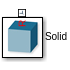
\includegraphics[width=0.75\textwidth]{sm_solid}
        \caption{Ciało stałe.}
        \label{fig:sm_solid}
    \end{subfigure}
    ~ 
    \begin{subfigure}[t]{0.2\textwidth}
        \centering
        
\includegraphics[width=0.75\textwidth]{sm_rigid_transform}
        \caption{Transformacja układu odniesienia.}
        \label{fig:sm_rigid_transform}
    \end{subfigure}
    ~ 
    \begin{subfigure}[t]{0.2\textwidth}
        \centering
        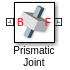
\includegraphics[width=0.75\textwidth]{sm_prismatic_joint}
        \caption{Złącze pryzmatyczne.}
        \label{fig:sm_prismatic_joint}
    \end{subfigure}
    ~
    \begin{subfigure}[t]{0.2\textwidth}
        \centering
        
\includegraphics[width=0.75\textwidth]{sm_revolute_joint}
        \caption{Złącze obrotowe.}
        \label{fig:sm_revolute_joint}
    \end{subfigure}
    
    \caption{Podstawowe bloki budujące schemat \textsc{SimMechanics}.}
    \label{fig:simmechanics_bloki}
\end{figure}

Budowanie schematu z wykorzystaniem bloków \textsc{SimMechanics} polega na, w dużym uproszczeniu, przyłączaniu ciał stałych w centrach układów odniesienia, które przemieszczane są w przestrzeni za pomocą bloków \textit{Rigid Transform} (rys. \ref{fig:sm_rigid_transform}). Wspomniane bloki umożliwiają również rotację układów odniesienia, co jest często konieczne do poprawnego działania złącz o pewnej liczbie stopni swobody. Przykładowo, złącze \textit{Revolute Joint} (\cref{fig:sm_revolute_joint}) umożliwia obracanie układu odniesienia \texttt{F} (ang. \textit{Follower} --- następujący układ odniesienia) wokół osi Z~układu \texttt{B} (ang. \textit{Base} --- poprzedzający układ odniesienia)\footnote{W ustawieniach bloku \textit{Revolute Joint} możliwa jest zmiana na tryb odwrotny, tj. obrót układu \texttt{B} wokół układu \texttt{F}.}. Jednakże jeśli wał, który ma się obracać wokół swojej naturalnej osi obrotu, nie ma w swoim układzie osi Z~wzdłuż naturalnej osi obrotu, wtedy jego układ odniesienia musi zostać transformowany za pomocą \textit{Rigid Transform}.

Bloki złącz umożliwiają pozyskanie informacji o aktualnych wartościach pozycji, prędkości i przyspieszenia (w zależności od typu złącza odpowiednio liniowych lub obrotowych) oraz przyłożonego na złącze momentu obrotowego lub siły. Dodatkowo możliwe jest załączenie wejścia momentu oddziałującego lub siły, co zostało wykorzystane przy implementacji silnika.

Ostatnią wartą wspomnienia informacją jest możliwość ustawienia pewnej wartości wstępnej dla danego złącza (warunku początkowego). W przypadku złącza \textit{Revolute Joint} umożliwia to wymuszenie kąta obrotu pomiędzy układami odniesienia \texttt{B} oraz \texttt{F}, a w przypadku złącza \textit{Prismatic Joint} wymusza to odpowiednie przesunięcie.

\section{Reprezentacja obiektu typu kulka i belka}
\label{sec:ch4_reprezentacja_obiektu_kulka_i_belka}

Bardzo dużą zaletą korzystania z \textsc{SimMechanics} jest automatyczne generowanie podglądu i animacji (zob. \cref{fig:uklad_simmechanics}) budowanego układu. Pozwala to przeprowadzać obserwację działania różnych algorytmów sterowania oraz łatwo znajdować błędy złożenia brył.

\begin{figure}[h]
    \centering
    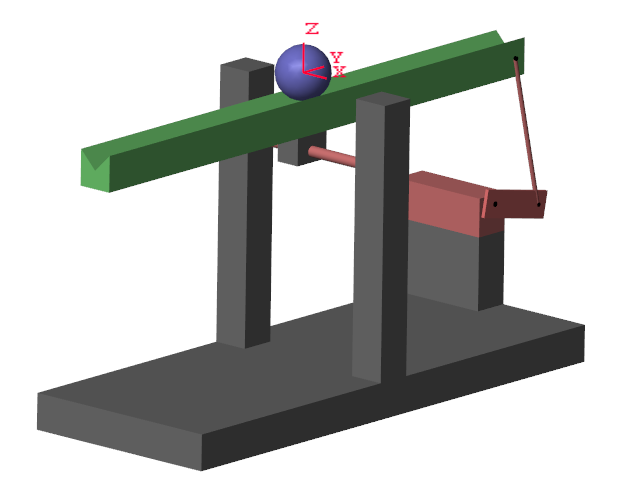
\includegraphics[width=0.5\textwidth]{simmechanics_ballandbeam}
    \caption{Wizualizacja układu kulki i belki zamodelowanego przy pomocy \textsc{SimMechanics} (por. z obiektem rzeczywistym przedstawionym na \cref{fig:perspektywa}).}
    \label{fig:uklad_simmechanics}
\end{figure}

Schemat użyty do wygenerowania modelu z \cref{fig:uklad_simmechanics} został przedstawiony na \cref{fig:uklad_simmechanics2}. Poczynając od lewej strony, możemy na nim wyróżnić kilka charakterystycznych elementów:

\begin{itemize}
    \item obiekty \textit{Base}, \textit{Tower1}, \textit{Tower2}, \textit{MotorBase}, \textit{Shaft Supports}, \textit{Motor}, \textit{Beam}, \textit{Pin2}, \textit{Ball} oraz \textit{CrankShaft},
    \item podsystemy \textit{Shaft}, \textit{Electric Motor}, \textit{Crank} oraz \textit{Ball mechanics},
    \item sporo bloków \textit{Rigid Transform} o nazwach \textit{RT}---\textit{RT19},
    \item trzy bloki \textit{Revolute Joint},
    \item wejścia \textit{voltage} oraz \textit{disturbance},
    \item wyjścia \textit{ball\_position}, \textit{ball\_velocity}, \textit{beam\_angle} oraz \textit{beam\_angular\_velocity}.
\end{itemize}

Obiekt \textit{Base} reprezentuje podstawę, na której umieszczono całą mechanikę układu. Poprzez transformacje \textit{RT} oraz \textit{RT1} umieszczono na nim dwa słupy, na których zaczepione są łożyska i wał obrotowy belki (podsystem \textit{Shaft}, \cref{fig:sm_shaft}).

Wał belki składa się z dwóch równoległych ścieżek, transformowanych z globalnego układu odniesienia poprzez bloki \textit{RT2} oraz \textit{RT3}. Za blokami umieszczono złącza obrotowe \textit{BallBearing1} oraz \textit{BallBearing2}, reprezentujące fizyczne łożyska kulkowe (zob. rozdział \ref{sec:ch2_konstrukcja_mechaniczna}). Złącze \textit{BallBearing2} zostało wykorzystane do pobrania z układu aktualnego kąta oraz prędkości kątowej obrotu belki.

Idąc dalej, w odpowiednim przesunięciu od środka wału belki (\textit{RT6}) zamontowano podpory wału (\textit{Shaft Supports}) --- tutaj zamodelowane jako jeden obiekt. Na nich (\textit{RT7}) została przymocowana belka, której kształt w przekroju przypomina domkniętą i wypełnioną literę \texttt{M}.

Na schemacie układu \ref{fig:uklad_simmechanics2} równolegle do ,,górnej'' części obiektu (wał belki, belka, kulka) poprowadzona jest ścieżka silnika i przekładni korbowej; obie ścieżki złączone są poprzez korbowód (\textit{Crankshaft}).

\begin{sidewaysfigure}[p!]
    \centering
    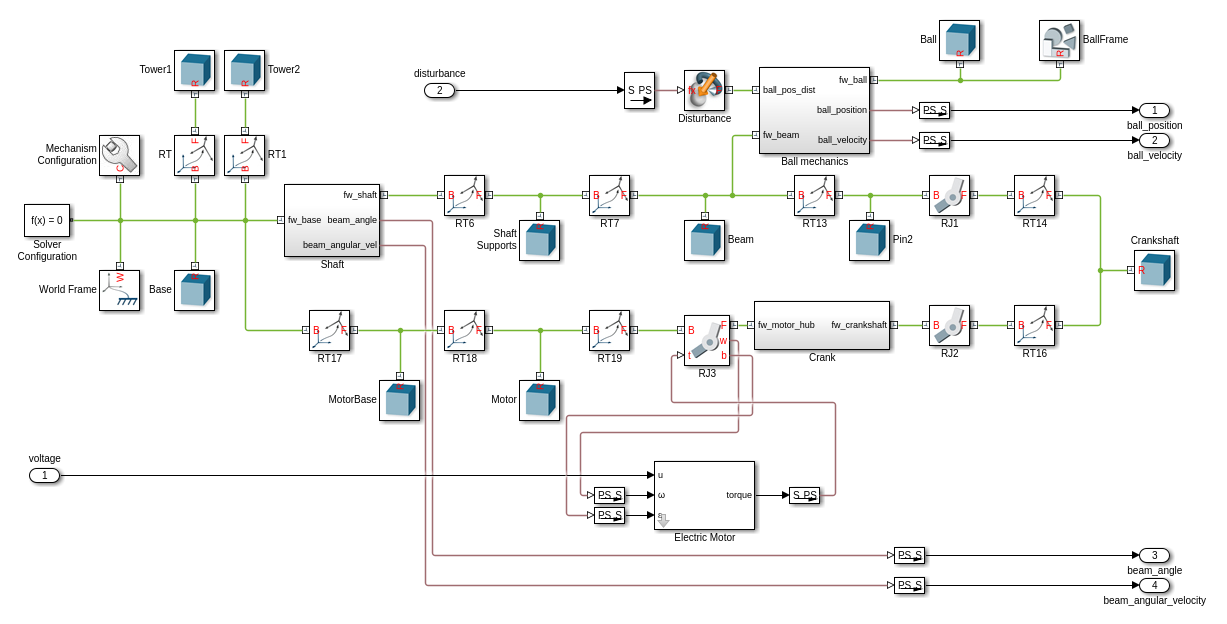
\includegraphics[width=\textwidth]{simmechanics_ballandbeam2}
    \caption{Schemat \textsc{SimMechanics} układu kulki i belki.}
    \label{fig:uklad_simmechanics2}
\end{sidewaysfigure}

Obiekty \textit{MotorBase} oraz \textit{Motor} reprezentują bryły podstawy, na której osadzony jest silnik oraz silnika. Elementy te nie biorą udziału w ogólnym zachowaniu belki pod wpływem momentu generowanego przez silnik, wobec czego nie nadano im skomplikowanych kształtów, jakie te elementy mają w~rzeczywistości.

\begin{figure}[h]
    \centering
    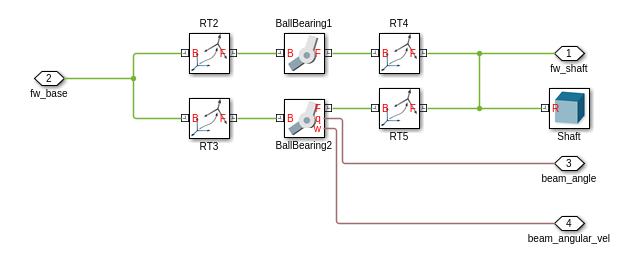
\includegraphics[width=0.8\textwidth]{simmechanics_shaft}
    \caption{Schemat podsystemu \textit{Shaft} odpowiadającego za umocowanie wału obrotu belki w danym układzie odniesienia.}
    \label{fig:sm_shaft}
\end{figure}

Sposób wykorzystania złącza obrotowego \textit{RJ3} został opisany w rozdziale \ref{sec:ch4_model_silnika}. Za wspomnianym złączem znajduje się podsystem \textit{Crank} (przedstawiony na \cref{fig:sm_shaft}), który składa się głównie z dwóch czarnych pinów (elementów mocujących o zerowej masie --- masa fizycznych przegubów włączona jest do masy korby bądź korbowodu) i korby (\textit{Crank}).

\begin{figure}[h]
    \centering
    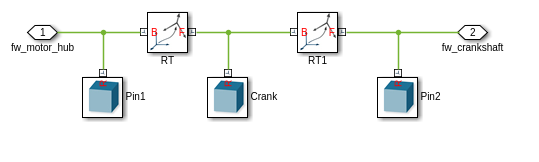
\includegraphics[width=0.8\textwidth]{simmechanics_crank}
    \caption{Schemat podsystemu \textit{Crank} odpowiadającego za umocowanie korby na wale motoreduktora.}
    \label{fig:sm_crank}
\end{figure}

Ostatnim, nieopisanym dotąd podsystemem, jest \textit{Ball mechanics} --- podsystem połączony z belką (\cref{fig:sm_ball_mechanics}), którego zadaniem jest ,,przytwierdzenie'' kulki do belki; osiągnięto to za pomocą nieopisanego dotąd bloku \textit{Rack and pinion} (pol. \textit{listwa (zębatka) współpracująca z kołem zębatym}).

Blok \textit{Rack and pinion} wymaga dla poprawnej pracy uzupełniania o dodatkowe elementy, na przykład w postaci złącz pryzmatycznego i obrotowego. Reprezentuje on więzy dla ruchu obrotowo-postępowego, z zerowym tarciem i~z~brakiem oderwania pod wpływem przyspieszeń pionowych, co dobrze przybliża zachowanie kulki w~układzie kulki i belki.

Połączenie równoległe bloków \textit{RPC1} i \textit{PJ}, \textit{RJ} przedstawione na \cref{fig:sm_ball_mechanics} spowodowane jest wymaganiami bloku \textit{Rack and pinion} co do osi przesuwu i osi obrotu; z tego powodu konieczne było użycie odpowiednich transformacji układów odniesienia \textit{RT12} oraz \textit{RT11}.

\begin{figure}[h]
    \centering
    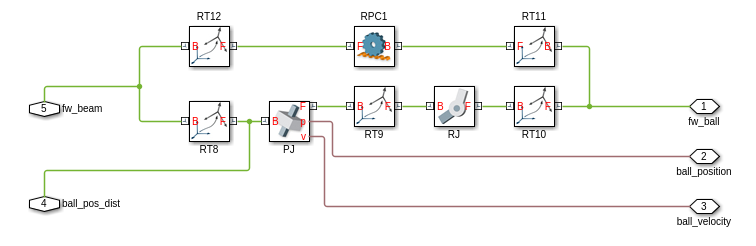
\includegraphics[width=0.9\textwidth]{simmechanics_ball_mechanics}
    \caption{Schemat podsystemu \textit{Ball mechanics} odpowiadającego za zachowanie kulki na belce.}
    \label{fig:sm_ball_mechanics}
\end{figure}

W układzie na \cref{fig:uklad_simmechanics2} jedno z wejść, oznaczone jako \textit{disturbance}, przeznaczone jest na symulowanie zewnętrznych zakłóceń wpływających bezpośrednio na kulkę; widoczne jest to w schemacie \textit{Ball mechanics} jako wejście \textit{ball\_pos\_dist}.

Z podsystemu \textit{Ball mechanics} wychodzą również dwa wyjścia: \textit{ball\_position} oraz \textit{ball\_velocity}. Odczytywane są one ze złącza pryzmatycznego kulki \textit{PJ}.

Sama kulka została dołączona do schematu poza podsystemem \textit{Ball mechanics}, jako ciało stałe \textit{Ball}. Równolegle dołączony blok \textit{BallFrame} odpowiada za wyświetlenie wersorów układu odniesienia środka kulki, co pomaga zobaczyć na wizualizacji faktyczny ruch obrotowy kulki po belce.

\section{Model silnika}
\label{sec:ch4_model_silnika}

Widoczny na \cref{fig:sm_electric_motor} model silnika prądu stałego odpowiada modelowi matematycznemu opartemu o równanie elektryczne obwodu silnika \eqref{eq:silnik_r_el} i równanie mechaniczne dla mas wirujących \eqref{eq:silnik_r_mech} (\cite{SILNIKIEL}):

\begin{equation}\label{eq:silnik_r_el}
    u - R i - L \deriv{i}{t} = K \omega 
\end{equation}
\begin{equation}\label{eq:silnik_r_mech}
    T = K i - J \epsilon - \beta \omega - b \sgn \omega
\end{equation}
gdzie:
\begin{itemize}
    \item $u$ --- napięcie sterujące,
    \item $R$ --- rezystancja silnika,
    \item $i$ --- prąd w obwodzie twornika,
    \item $K$ --- stała elektryczna bądź mechaniczna silnika (w jednostkach \si{\volt\second\per\radian} lub \si{\newton\meter\per\ampere}),
    \item $L$ --- indukcyjność silnika (w modelu na \cref{fig:sm_electric_motor} przyjęta za zerową),
    \item $T$ --- moment generowany przez silnik,
    \item $J$ --- moment bezwładności sprowadzony na wał motoreduktora,
    \item $\omega$ --- prędkość kątowa wału motoreduktora,
    \item $\epsilon = \deriv{\omega}{t}$ --- przyspieszenie kątowe wału motoreduktora,
    \item $\beta$ --- współczynnik tarcia wiskotycznego przekładni oraz silnika,
    \item $b$ --- współczynnik tarcia suchego przekładni oraz silnika.
\end{itemize}

\begin{figure}[h]
    \centering
    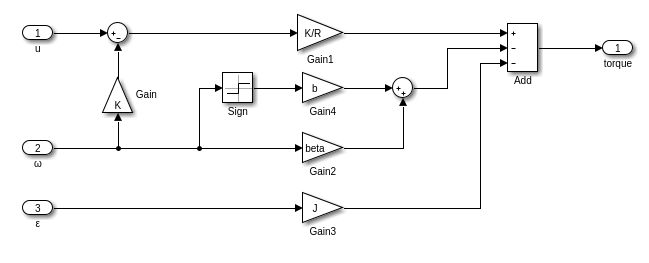
\includegraphics[width=0.8\textwidth]{simmechanics_electric_motor}
    \caption{Schemat podsystemu \textit{Electric Motor} odpowiadającego za model silnika prądu stałego.}
    \label{fig:sm_electric_motor}
\end{figure}

Warto zauważyć, że obliczanie kąta obrotu, prędkości kątowej oraz przyspieszenia kątowego odbywa się poza blokiem \textit{Electric Motor} --- wykonuje to \textsc{SimScape}, biorąc pod uwagę dynamikę reszty układu oraz moment, którym silnik działa na cały mechanizm.

W modelu silnika pominięto indukcyjność, gdyż jej wartość w rzeczywistości jest bardzo niska. Dodatkowo, przeprowadzona identyfikacja tarcia (rozdział \ref{sec:ch5_identyfikacja_parametrow_silnika}) pokazała, że poza tarciem mokrym w~układzie występuje pewne tarcie suche. Z powodu pracy silnika w sposób powtarzalny, tarcie suche może mieć spory wpływ na odpowiedź silnika, dlatego zdecydowano się go nie pomijać.

\section{Aproksymacja zależności kąta obrotu wału motoreduktora i osi belki}
\label{sec:ch4_zaleznosc_kata_silnika_i_kata_belki}

W związku z brakiem czujnika kąta obrotu wału belki, do odczytania jej położenia należy się posłużyć zależnością geometryczną od kąta obrotu wału motoreduktora. W rozdziale \ref{sec:ch3_uklad_napedowy} zasygnalizowano, że w pewnych niewielkich odchyleniach zależność ta może być opisana wzorem $\theta = \frac{L}{d_k} \alpha$.

Model symulacyjny \textsc{SimMechanics} eliminuje to ograniczenie, gdyż pozycja i prędkość wału belki odczytywane są bezpośrednio ze złącza obrotowego, w którym osadzony jest wspomniany wał. Niemniej jednak problem nadal występuje w rzeczywistym układzie, ponieważ nie zastosowano tam żadnego czujnika pozycji kątowej belki. Stąd postanowiono zmierzyć zależność $\theta(\alpha)$ poprzez symulację zbudowanego modelu. W tym celu podano stałe sterowanie na silnik i zmierzono jednocześnie kąt obrotu wału motoreduktora i wału belki.

\begin{figure}[h]
    \centering
    \includesvg[width=0.9\textwidth,svgpath=./vector_graphics/]{zaleznosc_kata2}
    \caption{Zależność kąta obrotu wału belki od kąta obrotu wału motoreduktora.}
    \label{fig:zaleznosc_kata_belki_od_enkodera}
\end{figure}

Należy zauważyć, że brak dobranych poprawnie parametrów silnika lub kulki nie wpływa negatywnie na dokładność aproksymacji, gdyż elementy łączące belkę z silnikiem są sztywne, a pomiar nie dotyczył dynamiki (prędkość, przyspieszenie) lecz statyki (obrót).

Obrót belki w funkcji obrotu wału motoreduktora postanowiono aproksymować sinusoidą (\cref{fig:zaleznosc_kata_belki_od_enkodera}) o następującym wzorze:
\begin{equation}\label{eq:aproksymacja_kata_walu}
    \theta(\alpha) = A \sin (\omega \alpha + \phi) + B
\end{equation}
gdzie:
\begin{itemize}
    \item $A$ --- amplituda sinusoidy,
    \item $\omega$ --- pulsacja,
    \item $\phi$ --- przesunięcie fazowe,
    \item $B$ --- wyraz wolny.
\end{itemize}

%Dane otrzymane po przeprowadzeniu aproksymacji numerycznej za pomocą funkcji \texttt{fminsearch} z programu \textsc{Matlab} pokazały, że kąt obrotu belki nie jest funkcją 
%Po przeprowadzeniu aproksymacji numerycznej za pomocą funkcji \texttt{fminsearch} z programu \textsc{Matlab} otrzymano 
Po przeprowadzeniu aproksymacji numerycznej za pomocą funkcji \texttt{fminsearch} z programu \textsc{Mat\-lab} otrzymano następujące wartości parametrów funkcji \eqref{eq:aproksymacja_kata_walu}: $A = \num{0.2387}$, $\omega = \num{1.0014}$, $\phi = \num{-1.5484}$, $B = \num{-0.05655}$; przybliżenie zostało przedstawione na \cref{fig:zaleznosc_kata_belki_od_enkodera}. Taka funkcja nie jest trudna do implementacji na sterowniku PLC, nie powinna również stanowić zbyt dużego wyzwania obliczeniowego\footnote{Producent deklaruje min. \SI{18}{\micro\second} dla obliczeń zmiennoprzecinkowych.} dla wybranego procesora (zob. tabelę \ref{tab:parametry_PLC_SB}).

Należy zauważyć, że wykres rzeczywistego kąta obrotu belki na \cref{fig:zaleznosc_kata_belki_od_enkodera} ma taki sam okres, jak wykres przybliżenia sinusoidą, a jednak kształt nie odpowiada mu całkowicie. Nie jest to błędem, gdyż w związku z działaniem w punkcie równowagi (zob. rozdział \ref{cha:ch6_model_liniowy}) największa dokładność przybliżenia oczekiwana jest w otoczeniu \SI[quotient-mode = fraction]{\pi/2}{\radian} kąta obrotu wału, czyli tam, gdzie oba wykresy są zbliżone.

\section{Podsumowanie}

W niniejszym rozdziale opisano sposób budowy modeli za pomocą przybornika narzędziowego \textsc{Simscape Multibody}, następnie przedstawiono i omówiono zbudowany w ten sposób model symulacyjny obiektu regulacji. W kolejnej części opisano model matematyczny silnika prądu stałego i jego implementację. Na końcu zaprezentowano wykorzystanie modelu obiektu do znalezienia zależności geometrycznej między kątem obrotu wału motoreduktora i wału belki.

%---------------------------------------------------------------------------